% This template has been tested with IEEEtran of 2015.

% !TeX spellcheck = es
% LTeX: language=es
% !TeX encoding = utf8
% !TeX program = lualatex
% !BIB program = bibtex
% -*- coding:utf-8 mod:LaTeX -*-

% DO NOT DOWNLOAD IEEEtran.cls - Use the one of your LaTeX distribution
\documentclass[conference,a4paper]{IEEEtran}[2015/08/26]

% Balance the last page (disabled - requires full TeX Live)
% \usepackage{pbalance}

\usepackage{iftex}

% backticks (`) are rendered as such in verbatim environments.
% See following links for details:
%   - https://tex.stackexchange.com/a/341057/9075
%   - https://tex.stackexchange.com/a/47451/9075
%   - https://tex.stackexchange.com/a/166791/9075
\usepackage{upquote}

% Idioma español como principal
\usepackage[english,main=spanish]{babel}
\addto\captionsspanish{\renewcommand{\tablename}{Tabla}}
\addto\captionsspanish{\renewcommand{\abstractname}{Resumen}}

% Links behave as they should. Enables "\url{...}" for URL typesettings.
% Allow URL breaks also at a hyphen, even though it might be confusing: Is the "-" part of the address or just a hyphen?
% See https://tex.stackexchange.com/a/3034/9075.
\usepackage[hyphens]{url}

% When activated, use text font as url font, not the monospaced one.
% For all options see https://tex.stackexchange.com/a/261435/9075.
% \urlstyle{same}

% Improve wrapping of URLs - hint by http://tex.stackexchange.com/a/10419/9075
\makeatletter
\g@addto@macro{\UrlBreaks}{\UrlOrds}
\makeatother

% nicer // - solution by http://tex.stackexchange.com/a/98470/9075
% DO NOT ACTIVATE -> prevents line breaks
%\makeatletter
%\def\Url@twoslashes{\mathchar`\/\@ifnextchar/{\kern-.2em}{}}
%\g@addto@macro\UrlSpecials{\do\/{\Url@twoslashes}}
%\makeatother

%% !!! If you change the font, be sure that words such as "workflow" can
%% !!! still be copied from the PDF. If this is not the case, you have
%% !!! to use glyphtounicode. See comment at cmap package.
%%
%% Background: "workflow" contains "fl" which is a ligature, which in turn
%%             is rendered as one character in the PDF and needs to be split
%%             whily copying.

\ifluatex
  \usepackage[no-math]{fontspec}
  \usepackage{unicode-math}

  % Enable proper ligatures
  % For more information see https://ctan.org/pkg/selnolig
  % language "english" or "ngerman" is passed to selnolig by the document class
  \usepackage{selnolig}

\else
  % use nicer font for code
  \usepackage[zerostyle=b,scaled=.75]{newtxtt}

  % Has to be loaded AFTER any font packages. See https://tex.stackexchange.com/a/2869/9075.
  \usepackage[T1]{fontenc}
\fi

% Character protrusion and font expansion. See http://www.ctan.org/tex-archive/macros/latex/contrib/microtype/

\usepackage[
  babel=true, % Enable language-specific kerning. Take language-settings from the languge of the current document (see Section 6 of microtype.pdf)
  expansion=alltext,
  protrusion=alltext-nott, % Ensure that at listings, there is no change at the margin of the listing
  % In the standard configuration, this template is always in the final mode, so this option only makes a difference if "pros" use the draft mode
  final % Always enable microtype, even if in draft mode. This helps finding bad boxes quickly.
]{microtype}

% \texttt{test -- test} keeps the "--" as "--" (and does not convert it to an en dash)
\DisableLigatures{encoding = T1, family = tt* }

%\DeclareMicrotypeSet*[tracking]{my}{ font = */*/*/sc/* }%
%\SetTracking{ encoding = *, shape = sc }{ 45 }
% Source: http://homepage.ruhr-uni-bochum.de/Georg.Verweyen/pakete.html
% Deactiviated, because does not look good

\usepackage{graphicx}

% Diagonal lines in a table - http://tex.stackexchange.com/questions/17745/diagonal-lines-in-table-cell
% Slashbox is not available in texlive (due to licensing) and also gives bad results. Thus, we use diagbox
\usepackage{diagbox}

\ifluatex
  \usepackage{spelling}
  \spellingoutput{off}
\fi

\usepackage[dvipsnames, table]{xcolor}
% Code Listings
\usepackage{listings}

\definecolor{eclipseStrings}{RGB}{42,0.0,255}
\definecolor{eclipseKeywords}{RGB}{127,0,85}
\colorlet{numb}{magenta!60!black}

% JSON definition
% Source: https://tex.stackexchange.com/a/433961/9075

\lstdefinelanguage{json}{
  basicstyle=\normalfont\ttfamily,
  commentstyle=\color{eclipseStrings}, % style of comment
  stringstyle=\color{eclipseKeywords}, % style of strings
  numbers=left,
  numberstyle=\scriptsize,
  stepnumber=1,
  numbersep=8pt,
  showstringspaces=false,
  breaklines=true,
  frame=lines,
  % backgroundcolor=\color{gray}, %only if you like
  string=[s]{"}{"},
  comment=[l]{:\ "},
  morecomment=[l]{:"},
  literate=
    *{0}{{{\color{numb}0}}}{1}
    {1}{{{\color{numb}1}}}{1}
    {2}{{{\color{numb}2}}}{1}
    {3}{{{\color{numb}3}}}{1}
    {4}{{{\color{numb}4}}}{1}
    {5}{{{\color{numb}5}}}{1}
    {6}{{{\color{numb}6}}}{1}
    {7}{{{\color{numb}7}}}{1}
    {8}{{{\color{numb}8}}}{1}
    {9}{{{\color{numb}9}}}{1}
}

\lstset{
  % everything between (* *) is a latex command
  escapeinside={(*}{*)},
  %
  language=json,
  %
  showstringspaces=false,
  %
  basicstyle=\footnotesize\ttfamily,
  %
  commentstyle=\slshape,
  %
  % default: \rmfamily
  stringstyle=\ttfamily,
  %
  breaklines=true,            % Zeilen werden umbrochen
  %
  breakatwhitespace=true,
  %
  % alternative: fixed
  columns=flexible,
  %
  tabsize=2,                  % Groesse von Tabs
  %
  numbers=left,
  %
  numberstyle=\tiny,
  %
  basewidth=.5em,
  %
  xleftmargin=.5cm,
  %
  % aboveskip=0mm,
  %
  % belowskip=0mm,
  %
  captionpos=b
}

\ifpdftex
  % Enable Umlauts when using \lstinputputlisting.
  % See https://stackoverflow.com/a/29260603/873282 and https://tex.stackexchange.com/a/24532/9075 for details.
  % listingsutf8 did not work in June 2020.
  \lstset{extendedchars=true, literate=
    {á}{{\'a}}1 {é}{{\'e}}1 {í}{{\'i}}1 {ó}{{\'o}}1 {ú}{{\'u}}1
  {Á}{{\'A}}1 {É}{{\'E}}1 {Í}{{\'I}}1 {Ó}{{\'O}}1 {Ú}{{\'U}}1
  {à}{{\`a}}1 {è}{{\`e}}1 {ì}{{\`i}}1 {ò}{{\`o}}1 {ù}{{\`u}}1
  {À}{{\`A}}1 {È}{{\'E}}1 {Ì}{{\`I}}1 {Ò}{{\`O}}1 {Ù}{{\`U}}1
  {ä}{{\"a}}1 {ë}{{\"e}}1 {ï}{{\"i}}1 {ö}{{\"o}}1 {ü}{{\"u}}1
  {Ä}{{\"A}}1 {Ë}{{\"E}}1 {Ï}{{\"I}}1 {Ö}{{\"O}}1 {Ü}{{\"U}}1
  {â}{{\^a}}1 {ê}{{\^e}}1 {î}{{\^i}}1 {ô}{{\^o}}1 {û}{{\^u}}1
  {Â}{{\^A}}1 {Ê}{{\^E}}1 {Î}{{\^I}}1 {Ô}{{\^O}}1 {Û}{{\^U}}1
  {Ã}{{\~A}}1 {ã}{{\~a}}1 {Õ}{{\~O}}1 {õ}{{\~o}}1
  {œ}{{\oe}}1 {Œ}{{\OE}}1 {æ}{{\ae}}1 {Æ}{{\AE}}1 {ß}{{\ss}}1
  {ű}{{\H{u}}}1 {Ű}{{\H{U}}}1 {ő}{{\H{o}}}1 {Ő}{{\H{O}}}1
  {ç}{{\c c}}1 {Ç}{{\c C}}1 {ø}{{\o}}1 {å}{{\r a}}1 {Å}{{\r A}}1
  }
\fi

\lstloadlanguages{% Check dokumentation for further languages...
  %[Visual]Basic
  %Pascal
  %C
  %C++
  %XML
  %HTML
}

% For easy quotations: \enquote{text}
% This package is very smart when nesting is applied, otherwise textcmds (see below) provides a shorter command
\usepackage[autostyle=true]{csquotes}

% Enable using "`quote"' - see https://tex.stackexchange.com/a/150954/9075
\defineshorthand{"`}{\openautoquote}
\defineshorthand{"'}{\closeautoquote}

% Nicer tables (\toprule, \midrule, \bottomrule)
\usepackage{booktabs}

% Extended enumerate, such as \begin{compactenum}
\usepackage{paralist}

% Bibliopgraphy enhancements
%  - enable \cite[prenote][]{ref}
%  - enable \cite{ref1,ref2}
% Alternative: \usepackage{cite}, which enables \cite{ref1, ref2} only (otherwise: Error message: "White space in argument")

% Doc: http://texdoc.net/natbib
\usepackage[%
  square,        % for square brackets
  comma,         % use commas as separators
  numbers,       % for numerical citations;
  %sort           % orders multiple citations into the sequence in which they appear in the list of references;
  sort&compress  % as sort but in addition multiple numerical citations are compressed if possible (as 3-6, 15);
]{natbib}

% Same fontsize as without natbib
\renewcommand{\bibfont}{\normalfont\footnotesize}

% Enable hyperlinked author names in the case of \citet
% Source: https://tex.stackexchange.com/a/76075/9075
\usepackage{etoolbox}
\makeatletter
\patchcmd{\NAT@test}{\else \NAT@nm}{\else \NAT@hyper@{\NAT@nm}}{}{}
\makeatother

% Farbige Tabellen
% ----------------
% Das Paket colortbl wird inzwischen automatisch durch xcolor geladen
%
% Erweiterte Funktionen innerhalb von Tabellen
% --------------------------------------------
%%% Doc: http://mirror.ctan.org/tex-archive/macros/latex/contrib/multirow/multirow.sty
\usepackage{multirow} % Mehrfachspalten
%
%%% Doc: Documentation inside dtx Package
\usepackage{dcolumn}  % Ausrichtung an Komma oder Punkt

%%% Doc: http://mirror.ctan.org/tex-archive/macros/latex/contrib/supertabular/supertabular.pdf
%\usepackage{supertabular}

%%% Fussnoten/Endnoten ===================================================

% EN: Put footnotes below floats
% DE: Fußnoten unter Gleitumgebungen ("floats") platzieren
% Source: https://tex.stackexchange.com/a/32993/9075
\usepackage{stfloats}
\fnbelowfloat

% EN: Extended support for footnotes
% DE: Fußnoten
%
%\usepackage{dblfnote}  %Zweispaltige Fußnoten
%
% Keine hochgestellten Ziffern in der Fußnote (KOMA-Script-spezifisch):
%\deffootnote[1.5em]{0pt}{1em}{\makebox[1.5em][l]{\bfseries\thefootnotemark}}
%
% Abstand zwischen Fußnoten vergrößern:
%\setlength{\footnotesep}{.85\baselineskip}
%
% EN: Following command disables the separting line of the footnote
% DE: Folgendes Kommando deaktiviert die Trennlinie zur Fußnote
%\renewcommand{\footnoterule}{}
%
%\addtolength{\skip\footins}{\baselineskip} % Abstand Text <-> Fußnote

% DE: Fußnoten immer ganz unten auf einer \raggedbottom-Seite
% DE: fnpos kommt aus dem yafoot package
%\usepackage{fnpos}
%\makeFNbelow
%\makeFNbottom

% TODO (and comment) configuration
%
% - \todo (from todo, easy-todo, todonotes) / \TODO (from fixmetodonotes) - for "normal" TODOs
% - \todofix - "important" TODOs
%
% - \textcomment - highlights text and has a hover comment
% - \sidecomment - just puts a comment to the side. Note: \comment MUST NOT be used as command name, it is already defined by much packages (mathdesign, mindflow, verbatim, and others)
%
% - \missingfigure
%
% - \textmarker
% - \modified
% - \change      - adresses a review comment

% Enable nice comments
\usepackage{pdfcomment}

\newcommand{\textcomment}[2]{\colorbox{yellow!60}{#1}\pdfcomment[color={0.234 0.867 0.211},hoffset=-6pt,voffset=10pt,opacity=0.5]{#2}}

% Small PDF comment
% 1. Parameter: Comment
\newcommand{\sidecomment}[1]{\pdfcomment[color={0.045 0.278 0.643},voffset=4pt,icon=Note]{#1}}
% Disabled variant - for the final PDF
%\newcommand{\sidecomment}[1]{}

\newcommand{\todo}[1]{TODO!\sidecomment{#1}}

% Änderungen
%
% 1. Parameter: Review-Kommentar
% 2. Parameter: Neuer Text
\newcommand{\change}[2]{{\color{red}#2}\pdfcomment[color={0.234 0.867 0.211},voffset=8pt,opacity=0.5]{#1}}
% Disabled variant - for the final PDF
%\newcommand{\change}[2]{#2}

% Define default commands
\makeatletter
\@ifundefined{missingfigure}{\newcommand{\missingfigure}{... missing figure ...}}{}
\@ifundefined{textcomment}{\newcommand{\textcomment}[2]{#1 \todo{#2}}}{}
\@ifundefined{sidecomment}{\newcommand{\sidecomment}[1]{\marginpar{#1}}}{}
\@ifundefined{todo}{\newcommand{\todo}[1]{\sidecomment{#1}}}{}
\@ifundefined{TODO}{\newcommand{\TODO}[1]{\todo{#1}}}{}
\@ifundefined{todofix}{\newcommand{\todofix}[1]{\todo{#1}}}{}
\@ifundefined{change}{\newcommand{\change}[2]{#1 $\rightarrow$ #2}}{}
\makeatother

% Textmarker (Textfarbe rot)
\newcommand{\textmarker}[1]{{\color{red} #1}\xspace}

% Modified (Text blau)
\newcommand{\modified}[1]{{\color{blue!60!black} #1}\xspace}

\usepackage[group-minimum-digits=4,per-mode=fraction]{siunitx}

% Enable that parameters of \cref{}, \ref{}, \cite{}, ... are linked so that a reader can click on the number an jump to the target in the document
\usepackage{hyperref}

% Enable hyperref without colors and without bookmarks
\hypersetup{
  hidelinks,
  colorlinks=true,       % Links erhalten Farben statt Kaeten
  raiselinks=true,       % calculate real height of the link
  allcolors=black,
  pdfstartview=Fit,
  breaklinks=true,       % Links ueberstehen Zeilenumbruch
  hypertexnames=false,   % Fix jumping to algorithm line - http://tex.stackexchange.com/a/156404/9075
}

% Enable correct jumping to figures when referencing
\usepackage[all]{hypcap}

\usepackage[caption=false,font=footnotesize]{subfig}

% Alternative for making subfigures:
% Part of the caption package. See http://www.ctan.org/pkg/caption
% Ersetzt die Pakete subfigure und subfig - siehe https://tex.stackexchange.com/a/13778/9075
%
% (subfigure is outdated. subfig is maintained, but subcaption is better)
% See: http://tex.stackexchange.com/questions/13625/subcaption-vs-subfig-best-package-for-referencing-a-subfigure
%\usepackage[hypcap=true]{subcaption}

\usepackage[incolumn]{mindflow}

% Extensions for references inside the document (\cref{fig:sample}, ...)
% Enable usage \cref{...} and \Cref{...} instead of \ref: Type of reference included in the link
% That means, "Figure 5" is a full link instead of just "5".
\usepackage[capitalise,nameinlink,noabbrev]{cleveref}

\crefname{figure}{Figura}{Figuras}
\Crefname{figure}{Figura}{Figuras}
\crefname{table}{Tabla}{Tablas}
\Crefname{table}{Tabla}{Tablas}
\crefname{section}{Sección}{Secciones}
\Crefname{section}{Sección}{Secciones}
\crefname{listing}{Listado}{Listados}
\Crefname{listing}{Listado}{Listados}
\crefname{lstlisting}{Listado}{Listados}
\Crefname{lstlisting}{Listado}{Listados}

% lipsum, blindtext, mwe, currfile, tcolorbox removed (template examples deleted)

% MnSymbolC font removed (only used for \powerset in template examples)

% Allows for defining commands that don't eat spaces.
\usepackage{xspace}
% Adds compatibility to \xspace und \enquote
\makeatletter
\xspaceaddexceptions{\grqq \grq \csq@qclose@i \} }
\makeatother

\newcommand{\eg}{e.g.,\ }
\newcommand{\ie}{i.e.,\ }

% Enable hyphenation at other places as the dash.
% Example: applicaiton\hydash specific
\makeatletter
\newcommand{\hydash}{\penalty\@M-\hskip\z@skip}
% Definition of "= taken from http://mirror.ctan.org/macros/latex/contrib/babel-contrib/german/ngermanb.dtx
\makeatother

% Add manual adapted hyphenation of English words
% See https://ctan.org/pkg/hyphenex and https://tex.stackexchange.com/a/22892/9075 for details
\input{ushyphex}

% correct bad hyphenation here
\hyphenation{
  op-tical net-works semi-conduc-tor
  % May not be hypphenated
  AROMA TOSCA BPMN OASIS OMG DMTF IT DevOps
}

\input{commands}

\ifpdftex
  % Enable copy and paste of text from the PDF
  % Only required for pdflatex. It "just works" in the case of lualatex.
  % Alternative: cmap or mmap package
  % mmap enables mathematical symbols, but does not work with the newtx font set
  % See: https://tex.stackexchange.com/a/64457/9075
  % Other solutions outlined at http://goemonx.blogspot.de/2012/01/pdflatex-ligaturen-und-copynpaste.html and http://tex.stackexchange.com/questions/4397/make-ligatures-in-linux-libertine-copyable-and-searchable
  % Trouble shooting outlined at https://tex.stackexchange.com/a/100618/9075
  %
  % According to https://tex.stackexchange.com/q/451235/9075 this is the way to go
  \input{glyphtounicode}
  \pdfgentounicode=1
\fi
\begin{document}
% Enable following command if you need to typeset "IEEEpubid".
% See https://bytefreaks.net/tag/ieeeoverridecommandlockouts for details.
%\IEEEoverridecommandlockouts

\title{Detección de Productos en Tiempo Real para Autocobro usando YOLO11}

\author{%
  \IEEEauthorblockN{María Belén Cattaneo, Nicolás Valentín Ciarrapico, Sabrina Daiana Pryszczuk}
  \IEEEauthorblockA{Carrera de Especialización en Inteligencia Artificial\\
    Facultad de Ingeniería, Universidad de Buenos Aires\\
    Buenos Aires, Argentina}
}

% use for special paper notices
%\IEEEspecialpapernotice{(Invited Paper)}

% make the title area
\maketitle

% In case you want to add a copyright statement.
% Works only in the compsoc conference mode.
%
% Source: https://tex.stackexchange.com/a/325013/9075
%
% All possible solutions:
%  - https://tex.stackexchange.com/a/325013/9075
%  - https://tex.stackexchange.com/a/279134/9075
%  - https://tex.stackexchange.com/q/279789/9075 (TikZ)
%  - https://tex.stackexchange.com/a/200330/9075 - for non-compsocc papers
\iffalse
  \IEEEoverridecommandlockouts
  \IEEEpubid{\begin{minipage}{\textwidth}\ \\[12pt] \centering
      1551-3203 \copyright 2015 IEEE.
      Personal use is permitted, but republication/redistribution requires IEEE permission.
      \\
      See \url{https://www.ieee.org/publications_standards/publications/rights/index.html} for more information.
    \end{minipage}}
\fi

\begin{abstract}
Este trabajo presenta un sistema de detección y clasificación de productos en tiempo real orientado al autocobro en despensas comunitarias. El sistema utiliza YOLO11, seleccionado mediante un benchmark comparativo entre tres arquitecturas nano de la familia YOLO. Se construyó un dataset propio con 10 clases de productos típicos de despensa, capturados bajo condiciones controladas con vista cenital. El pipeline incorpora una lógica de registro estable basada en seguimiento multi-frame mediante Intersection over Union (IoU), que requiere $N$ detecciones consecutivas antes de confirmar un producto, reduciendo falsos positivos por variación de confianza entre cuadros. El modelo seleccionado (YOLO11n) obtuvo un mAP@0.5 de 0.967 en validación sobre producto individual y un mAP@0.5 de 0.946 en validación sobre escenas multi-producto, con inferencia en tiempo real superior a 15 FPS (Frames Per Second). La metodología propuesta es reproducible y extensible a catálogos de mayor escala. El código y el dataset se encuentran disponibles públicamente.\footnote{\url{https://github.com/BelCattaneo/vpc2_autocobro}}
\end{abstract}

% For peer review papers, you can put extra information on the cover
% page as needed:
% \ifCLASSOPTIONpeerreview
% \begin{center} \bfseries EDICS Category: 3-BBND \end{center}
% \fi
%
% For peerreview papers, this IEEEtran command inserts a page break and
% creates the second title. It will be ignored for other modes.
\IEEEpeerreviewmaketitle

\section{Introducción}
\label{sec:introduccion}

Las organizaciones comunitarias, como mutuales y cooperativas, frecuentemente gestionan despensas de bajo costo para sus asociados. En estos contextos, el cobro manual de productos implica tiempos de espera, errores de registro y dependencia de personal dedicado. Las soluciones comerciales de autocobro basadas en visión por computadora, como Amazon Go~\cite{amazongo}, requieren infraestructuras costosas y no están diseñadas para adaptarse a catálogos acotados y variables.

Los avances recientes en detección de objetos en tiempo real, impulsados por la familia de arquitecturas YOLO (You Only Look Once)~\cite{redmon2016yolo, redmon2018yolov3, wang2024yolov10}, han democratizado el acceso a modelos de alta precisión y baja latencia ejecutables en hardware de bajo costo. En el ámbito de productos de retail, el dataset RPC (Retail Product Checkout)~\cite{wei2019rpc} demostró la viabilidad del reconocimiento automático de productos en contextos de supermercado a gran escala. Más recientemente, Fuchs et al.~\cite{fuchs2019grocerystore} presentaron un sistema de reconocimiento de productos de supermercado basado en fine-tuning de redes convolucionales sobre un dataset propio de productos suecos, logrando accuracy superior al 85\% en un catálogo de 81 clases, demostrando la viabilidad del enfoque para catálogos acotados similares al de este trabajo.

Este trabajo propone un sistema de autocobro de bajo costo para despensas comunitarias, basado en la detección y clasificación de productos mediante fine-tuning de YOLO11~\cite{jocher2023ultralytics} sobre un dataset propio, seleccionado tras un benchmark comparativo entre variantes nano de YOLOv8, YOLOv10 y YOLO11. Las contribuciones principales son:
\begin{enumerate}
  \item Un pipeline reproducible para detección y registro de productos en tiempo real, con lógica de confirmación multi-frame que suprime falsos positivos sin necesidad de un tracker complejo.
  \item Un dataset propio de productos argentinos de despensa, capturado bajo condiciones controladas con cámara cenital, incluyendo escenas individuales y multi-producto con oclusiones parciales.
  \item Un análisis de rendimiento sobre clases visualmente similares (variantes de leche y aceite), que valida la capacidad de discriminación fina del modelo en condiciones de prueba de concepto.
  \item Una metodología extensible y documentada, que permite escalar el catálogo sin cambios en la arquitectura del sistema.
\end{enumerate}

El resto del trabajo está organizado de la siguiente manera: la \cref{sec:trabajos-relacionados} presenta los trabajos relacionados. La \cref{sec:metodologia} describe la metodología propuesta, incluyendo el dataset, modelo y pipeline de inferencia. La \cref{sec:experimentos} presenta los experimentos realizados y sus resultados. La \cref{sec:discusion} discute la interpretación de los resultados, limitaciones y trabajo futuro. Finalmente, la \cref{sec:conclusiones} presenta las conclusiones.

%% ===========================================================================
\section{Trabajos Relacionados}
\label{sec:trabajos-relacionados}

\subsection{Detección de Objetos}

La detección de objetos evolucionó desde arquitecturas two-stage, como R-CNN (Region-based Convolutional Neural Network)~\cite{girshick2014rcnn}, que separan la propuesta de regiones de su clasificación, hacia enfoques single-stage que unifican ambas etapas en una única pasada. La familia YOLO~\cite{redmon2016yolo} consolidó el paradigma single-stage al demostrar que la velocidad de inferencia y la precisión no son excluyentes. Versiones posteriores, como YOLOv3~\cite{redmon2018yolov3} y YOLOv4~\cite{bochkovskiy2020yolov4}, incorporaron mejoras en el backbone, la detección multi-escala y técnicas de data augmentation como mosaic. YOLOv10~\cite{wang2024yolov10} introduce un esquema de entrenamiento con asignaciones duales consistentes que elimina la necesidad de Non-Maximum Suppression (NMS) en tiempo de inferencia. La versión más reciente, YOLO11~\cite{jocher2023ultralytics}, mejora la eficiencia del backbone y alcanza el mejor balance entre precisión y velocidad en variantes nano, siendo la arquitectura seleccionada para este trabajo tras un benchmark comparativo (ver \cref{sec:experimentos}).

Como alternativa transformer-based, RT-DETR~\cite{zhao2023rtdetr} alcanza precisiones comparables con detección en tiempo real, pero con mayor complejidad computacional y requerimientos de memoria que lo hacen menos adecuado para hardware embebido de bajo costo.

\subsection{Detección de Productos en Retail}

El reconocimiento automático de productos en entornos de checkout presenta desafíos particulares: alta similaridad intra-clase (distintas marcas con envases parecidos), variabilidad de pose y oclusiones parciales en escenas con múltiples productos. El dataset RPC~\cite{wei2019rpc} es la referencia más citada en este dominio, con más de 83.000 imágenes y 200 categorías de productos de supermercado. Goldman et al.~\cite{goldman2019precise} abordaron la detección en escenas densamente agrupadas, relevante para contextos donde múltiples productos se superponen sobre una superficie.

A diferencia de estos trabajos, que asumen catálogos de escala masiva y datasets pre-existentes, este trabajo construye un dataset propio adaptado a los productos específicos de la despensa, priorizando la reproducibilidad sobre la escala.

\subsection{Sistemas de Autocobro}

Las soluciones comerciales de autocobro, como Amazon Go~\cite{amazongo}, combinan visión por computadora con sensores de peso y fusión de datos de múltiples cámaras para lograr una experiencia sin fricción. Su costo de implementación y la complejidad de infraestructura requerida las hace inaccesibles para organizaciones comunitarias pequeñas. El enfoque estándar de menor costo es el escaneo manual de códigos de barras, que elimina la automatización del reconocimiento pero evita los costos de infraestructura. Este trabajo propone un punto intermedio: un sistema basado exclusivamente en visión por computadora (CV) de bajo costo que automatiza el reconocimiento de productos sobre una superficie de control, sin requerir sensores adicionales ni servidores en la nube.

%% ===========================================================================
\section{Metodología}
\label{sec:metodologia}

\subsection{Arquitectura del Sistema}
\label{subsec:arquitectura}

El sistema se compone de cuatro etapas secuenciales (ver \cref{fig:arquitectura}): (1)~captura de video mediante cámara USB con vista cenital, (2)~inferencia con YOLO11 fine-tuneado sobre las clases del catálogo, (3)~lógica de registro estable que filtra y confirma detecciones a lo largo del tiempo, y (4)~salida dual: video anotado en tiempo real y archivo JSON con el estado de la mesa al finalizar la sesión.

\begin{figure}[htbp]
  \centering
  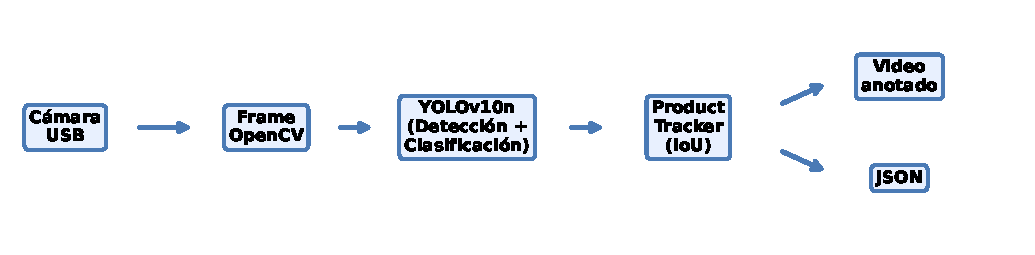
\includegraphics[width=\linewidth]{figures/arquitectura.pdf}
  \caption{Arquitectura del sistema de autocobro. El pipeline procesa cada frame de video a través de YOLO11n para detección y clasificación, aplica la lógica de registro estable basada en IoU, y genera una salida dual: video anotado en tiempo real y archivo JSON con el inventario final.}
  \label{fig:arquitectura}
\end{figure}

Se evaluó una arquitectura alternativa two-stage, con un detector genérico seguido de un clasificador especializado. Se descartó porque aproximadamente duplica la latencia de inferencia y agrega complejidad de mantenimiento sin beneficio en precisión para un catálogo acotado. El enfoque single-stage es suficiente para el dominio del problema y cumple con el requerimiento de tiempo real ($>$15~FPS).

El hardware de despliegue consiste en una Raspberry Pi~5 (8~GB) como dispositivo de cómputo, una webcam USB montada en posición cenital sobre la mesa de control, y un monitor conectado por HDMI que muestra el video anotado con la lista de productos en tiempo real. El costo total estimado del hardware es de 140--190~USD, significativamente inferior al de soluciones comerciales de autocobro.

\subsection{Dataset}
\label{subsec:dataset}

\subsubsection{Selección de Productos}

Se seleccionaron 10 clases de productos representativos del catálogo de la despensa comunitaria: aceite 1L, aceite 4L, dulce de leche, fideos, leche descremada, leche entera, miel, polenta, tomate y yerba. La selección incluye intencionalmente pares de productos visualmente similares (leche descremada/entera, aceite 1L/4L) para evaluar la capacidad de discriminación fina del modelo.

\subsubsection{Setup de Captura}

Las imágenes se capturaron con una webcam USB de 1080p montada en posición cenital a una distancia de 50--70~cm de la mesa de control. Se utilizó iluminación difusa para minimizar reflejos y un fondo uniforme para facilitar la segmentación. La configuración se mantuvo constante a lo largo de todas las sesiones de captura para garantizar consistencia en el dataset.

\subsubsection{Protocolo de Captura}

Se definieron múltiples tipos de escenas para capturar la variabilidad del caso de uso real: productos individuales (30--50 imágenes por clase), acumulaciones de 2--5 productos (20 escenas), acumulaciones de 5--10 productos (20 escenas), escenas con mano visible durante la colocación (10 escenas), y hard negatives con objetos que no pertenecen al catálogo (10 escenas). Adicionalmente, se grabaron videos de sesiones completas de checkout y se extrajeron frames con variación posicional para ampliar la diversidad del dataset.

\subsubsection{Anotación}

Las imágenes se anotaron mediante la plataforma Roboflow~\cite{roboflow2023} con bounding boxes en formato YOLO v5 PyTorch. Se realizó una revisión manual de las anotaciones para verificar la consistencia de las etiquetas y la precisión de las cajas delimitadoras. El dataset final comprende 296 imágenes anotadas: 127 en el dataset de producto individual (102 train, 13 val, 12 test) y 169 en el dataset multi-producto (132 train, 19 val, 18 test).

\subsubsection{Data Augmentation}

Se utilizaron las técnicas de data augmentation integradas en el framework Ultralytics~\cite{jocher2023ultralytics}, cuyas configuraciones por defecto han sido validadas extensivamente en la literatura de YOLO~\cite{bochkovskiy2020yolov4, shorten2019augmentation}. Las técnicas aplicadas incluyen: mosaic (probabilidad 1.0), que combina 4 imágenes de entrenamiento en una sola, incrementando la diversidad contextual; flip horizontal ($p=0.5$); y jitter de HSV (Hue, Saturation, Value; hue $= 0.015$, saturación $= 0.7$, valor $= 0.4$), que introduce variabilidad fotométrica. Adicionalmente, Roboflow aplicó auto-orientación y redimensionamiento a $640 \times 640$ píxeles con relleno por reflexión de bordes.

\subsubsection{División del Dataset}

El dataset se dividió en conjuntos de entrenamiento, validación y test. El dataset de producto individual contiene 102 imágenes de entrenamiento, 13 de validación y 12 de test. El dataset multi-producto contiene 132 imágenes de entrenamiento, 19 de validación y 18 de test (exportado desde Roboflow con división automática).

\subsection{Modelo}
\label{subsec:modelo}

\subsubsection{Selección de Arquitectura}

Se restringió la búsqueda a la familia YOLO por su balance comprobado entre precisión y latencia en hardware de bajo costo, descartando alternativas transformer-based como RT-DETR~\cite{zhao2023rtdetr} por su mayor complejidad computacional y requerimientos de memoria. Dentro de la familia YOLO, se evaluaron las variantes nano de tres generaciones --- YOLOv8n, YOLOv10n~\cite{wang2024yolov10} y YOLO11n~\cite{jocher2023ultralytics} --- mediante un benchmark comparativo sobre el dataset de producto individual (ver \cref{sec:experimentos}). YOLO11n fue seleccionado por ofrecer el mejor mAP@0.5:0.95 y la menor latencia de inferencia.

\subsubsection{Variante Seleccionada}

Se seleccionó la variante nano (YOLO11n, 2.5M parámetros) para cumplir con el requerimiento de inferencia en tiempo real ($>$15~FPS) incluso en hardware embebido como Raspberry Pi~5. La variante nano ofrece el mejor balance entre precisión y velocidad para el hardware objetivo.

\subsubsection{Configuración de Entrenamiento}

El modelo se entrenó mediante transfer learning~\cite{yosinski2014transferable} a partir de pesos pre-entrenados en COCO (Common Objects in Context), utilizando el framework Ultralytics~\cite{jocher2023ultralytics}. La configuración de entrenamiento fue: 100 épocas, batch size de 16, tamaño de imagen de $640 \times 640$ píxeles, y early stopping con paciencia de 20 épocas. Se utilizó el optimizador SGD (Stochastic Gradient Descent) con los hiperparámetros por defecto del framework (learning rate $= 0.01$, momentum $= 0.937$, weight decay $= 0.0005$). El entrenamiento se realizó en una laptop con Apple Silicon (backend MPS) con \texttt{amp=False} para evitar incompatibilidades con la precisión mixta en dicha plataforma.

\subsection{Pipeline de Inferencia}
\label{subsec:pipeline}

\subsubsection{Lógica de Registro Estable}

Para filtrar la variabilidad de confianza entre cuadros consecutivos, se implementó un algoritmo de registro multi-frame. Cada detección se asocia a un registro existente mediante IoU (Intersection over Union) con un umbral de $0.3$ y coincidencia de clase. Las detecciones no asociadas inician un nuevo registro en estado ``pendiente''. Un producto se confirma como presente en la mesa cuando ha sido detectado en al menos $N = 5$ frames consecutivos con confianza $\geq 0.5$. Los productos confirmados se mantienen registrados hasta que no se detectan durante $M = 10$ frames consecutivos, evitando des-registraciones prematuras por oclusiones momentáneas.

Adicionalmente, las detecciones con confianza entre $0.15$ y $0.5$ se muestran como ``advertencias'' en la interfaz (bounding boxes naranjas), alertando al usuario sobre productos potencialmente no reconocidos sin generar falsos positivos en el registro.

A 30~FPS, $N = 5$ frames equivale a $\sim$167~ms de detección consistente, tiempo suficiente para suprimir falsos positivos transitorios sin latencia perceptible para el usuario. El umbral de desaparición de $M = 10$ frames ($\sim$333~ms) permite oclusiones breves, como el paso de una mano sobre un producto.

\subsubsection{Tracking}

Se optó por un esquema de seguimiento simple basado en IoU en lugar de trackers más sofisticados como ByteTrack~\cite{zhang2022bytetrack}. La justificación es que el caso de uso involucra productos estacionarios acumulándose sobre una mesa: la predicción de movimiento basada en filtro de Kalman que utiliza ByteTrack agrega complejidad computacional sin beneficio para objetos estáticos. El problema a resolver no es la predicción de trayectorias, sino la confirmación estable de presencia a lo largo del tiempo.

\subsubsection{Visualización}

La interfaz de inferencia incluye un panel lateral de 250 píxeles que muestra la lista de productos confirmados con sus cantidades. Los bounding boxes se colorean según el estado: verde para productos confirmados, amarillo para detecciones pendientes de confirmación, y naranja para advertencias de baja confianza. Esta codificación permite al usuario del sistema verificar visualmente el estado del registro en tiempo real.

%% ===========================================================================
\section{Experimentos y Resultados}
\label{sec:experimentos}

\subsection{Configuración Experimental}

El entrenamiento y la evaluación se realizaron utilizando un procesador Intel Core i5-6200U sin aceleración gráfica dedicada (GPU), lo que permitió simular restricciones de hardware cercanas a las del entorno de producción. Las métricas de evaluación~\cite{everingham2010pascal} reportadas son: mean Average Precision a IoU $= 0.5$ (mAP@0.5) y a IoU $\in [0.5, 0.95]$ (mAP@0.5:0.95), precision media y recall medio sobre todas las clases.

\subsection{Benchmark de Arquitecturas (Prueba de Concepto - 10 clases)}

Para determinar el modelo óptimo a desplegar en la Raspberry Pi 5, se realizó una comparativa de rendimiento entre tres generaciones de arquitecturas ligeras: YOLOv8-Nano, YOLOv10-Nano y YOLO11-Nano. El entrenamiento se realizó sobre el dataset de producto individual (10 clases). Se intentó además entrenar una arquitectura basada en Transformers (RT-DETR-L), pero el proceso se abortó por saturación de memoria (Segmentation Fault), demostrando la inviabilidad de modelos pesados en este hardware. Los resultados de los modelos YOLO se presentan en la \cref{tab:resultados-benchmark}.

\begin{table}[htbp]
\centering
\caption{Comparativa de rendimiento en validación --- Dataset 10 clases.}
\label{tab:resultados-benchmark}
\begin{tabular}{lcccc}
\hline
\textbf{Modelo} & \textbf{Parámetros} & \textbf{Inferencia} & \textbf{mAP@0.5} & \textbf{mAP@0.5:0.95} \\
\hline
YOLOv8n & 3.0 M & 246.2 ms & \textbf{0.967} & 0.835 \\
YOLOv10n & \textbf{2.2 M} & 213.0 ms & 0.813 & 0.774 \\
YOLO11n & 2.5 M & \textbf{205.7 ms} & \textbf{0.967} & \textbf{0.889} \\
\hline
\end{tabular}
\end{table}

Los resultados indican que \textbf{YOLO11n} ofrece el mejor balance para el proyecto. Si bien empata con YOLOv8n en mAP@0.5, lo supera significativamente en la métrica más estricta (mAP@0.5:0.95), logrando además la mayor velocidad de inferencia por imagen. En consecuencia, YOLO11n es seleccionado como la arquitectura base para las siguientes etapas.

\subsection{Evaluación sobre Validation Split (YOLO11n)}

Se analizó en detalle el rendimiento del modelo seleccionado (YOLO11n) sobre el split de validación. La \cref{fig:confusion-matrix-val} muestra la matriz de confusión, donde se evidencia que las clases \textit{aceite\_1l}, \textit{polenta} y \textit{tomate} son detectadas con una precisión perfecta. 

\begin{figure}[htbp]
  \centering
  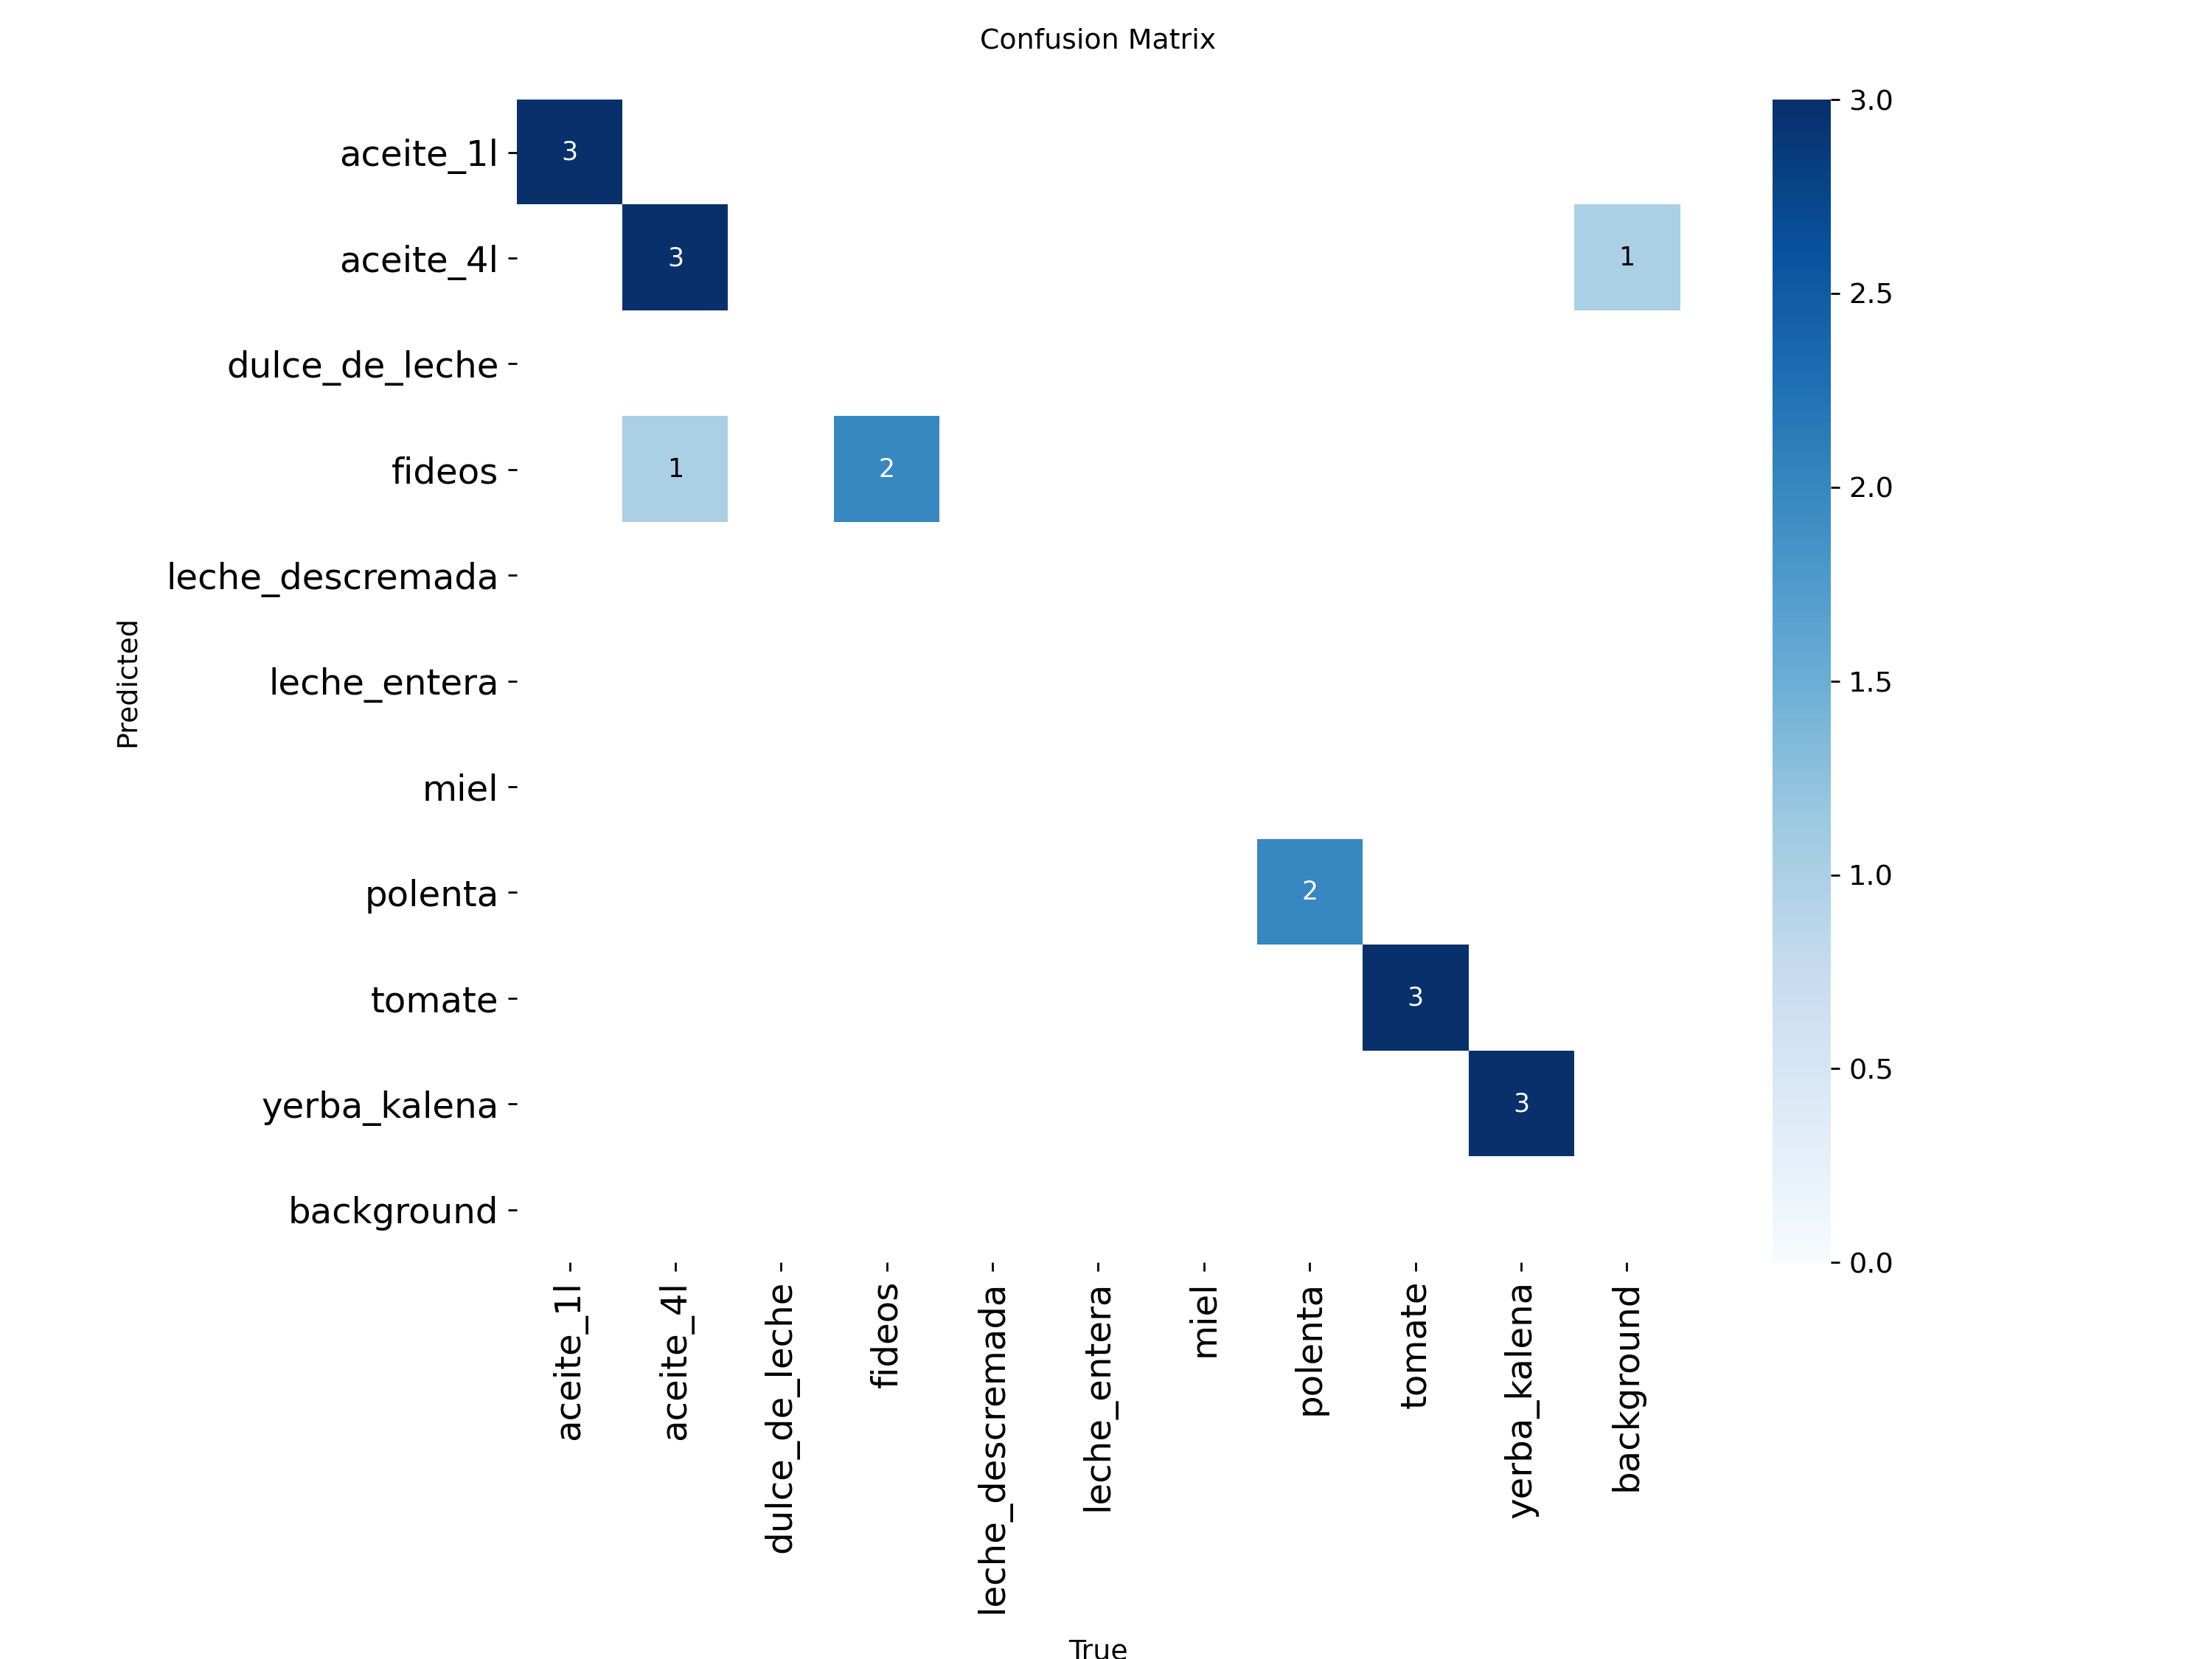
\includegraphics[width=\linewidth]{figures/confusion_matrix_val.png}
  \caption{Matriz de confusión para el modelo YOLO11n sobre el split de validación. Las filas representan las predicciones y las columnas el ground truth.}
  \label{fig:confusion-matrix-val}
\end{figure}

Por el contrario, la clase \textit{fideos} presenta cierta confusión. Evaluando las métricas por clase, \textit{fideos} obtuvo el mAP@0.5 más bajo con 0.828, marcando un fuerte contraste con el 0.995 obtenido por el resto de las clases detectadas de manera individual. 

La \cref{fig:pr-curve-val} presenta las curvas Precision-Recall, ilustrando la alta separabilidad visual en la mayoría de los productos y logrando el mAP@0.5 global de 0.967. 

\begin{figure}[htbp]
  \centering
  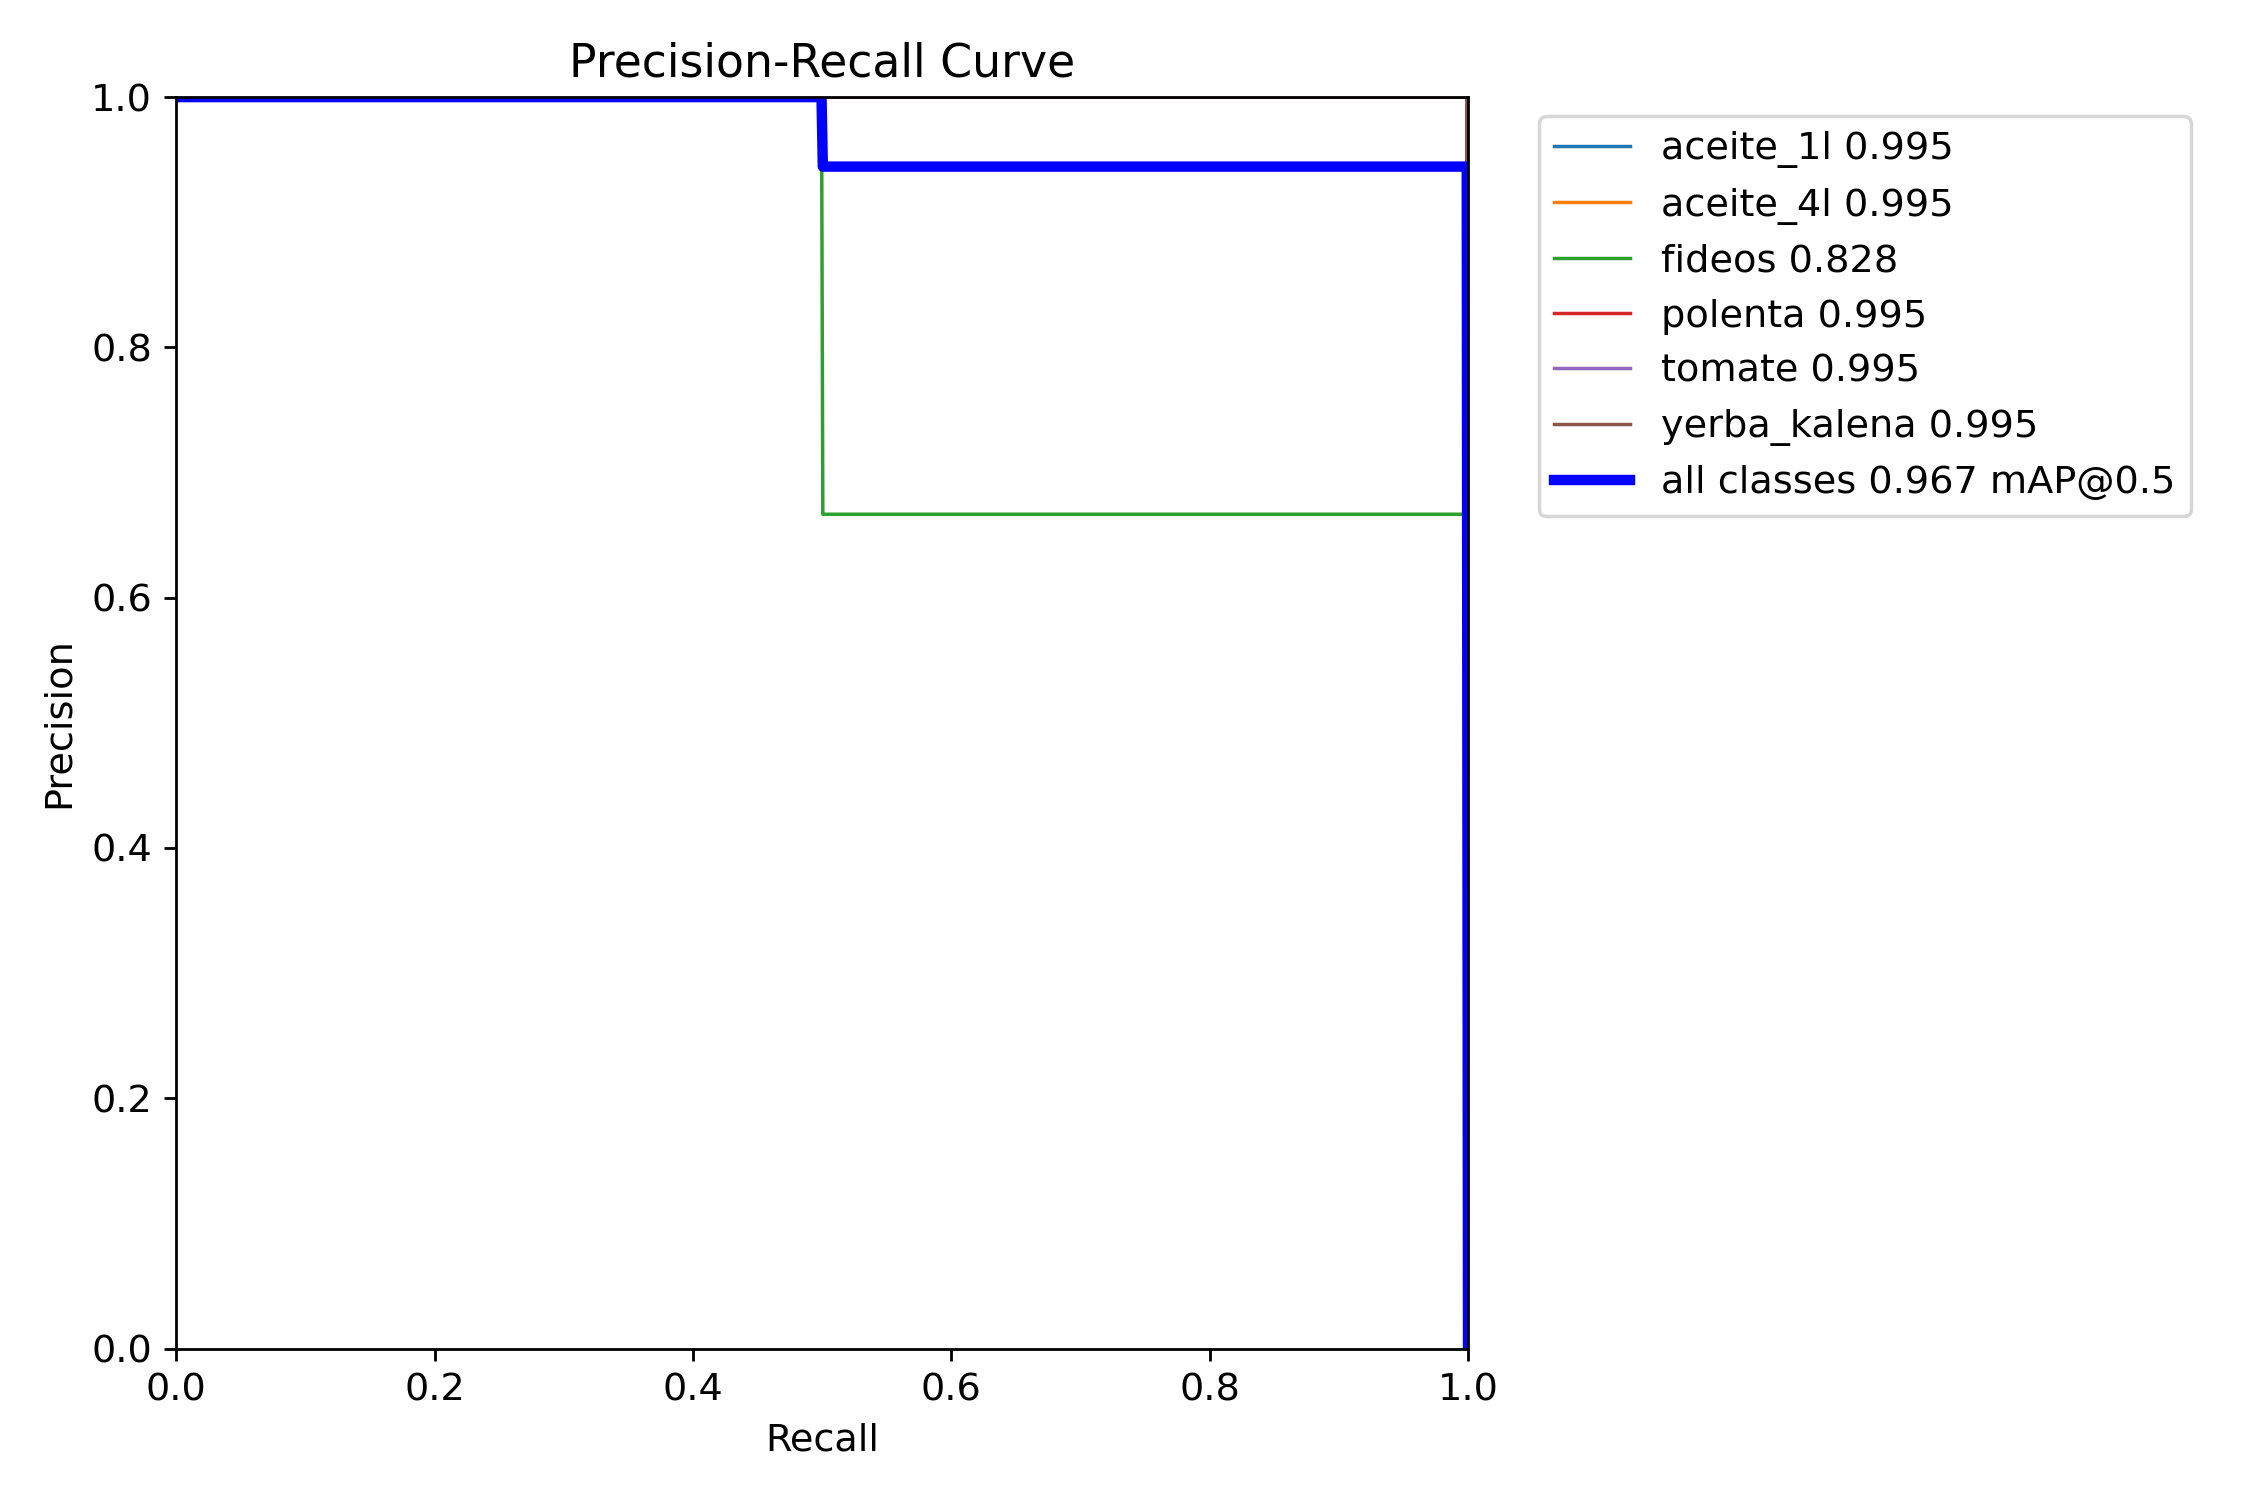
\includegraphics[width=\linewidth]{figures/BoxPR_curve_val.png}
  \caption{Curvas Precision-Recall por clase para el modelo YOLO11n. mAP@0.5 global = 0.967.}
  \label{fig:pr-curve-val}
\end{figure}

Finalmente, la \cref{fig:val-pred} ilustra predicciones cualitativas del modelo, evidenciando detecciones con altos niveles de confianza en la correcta ubicación espacial de los productos individuales.

\begin{figure}[htbp]
  \centering
  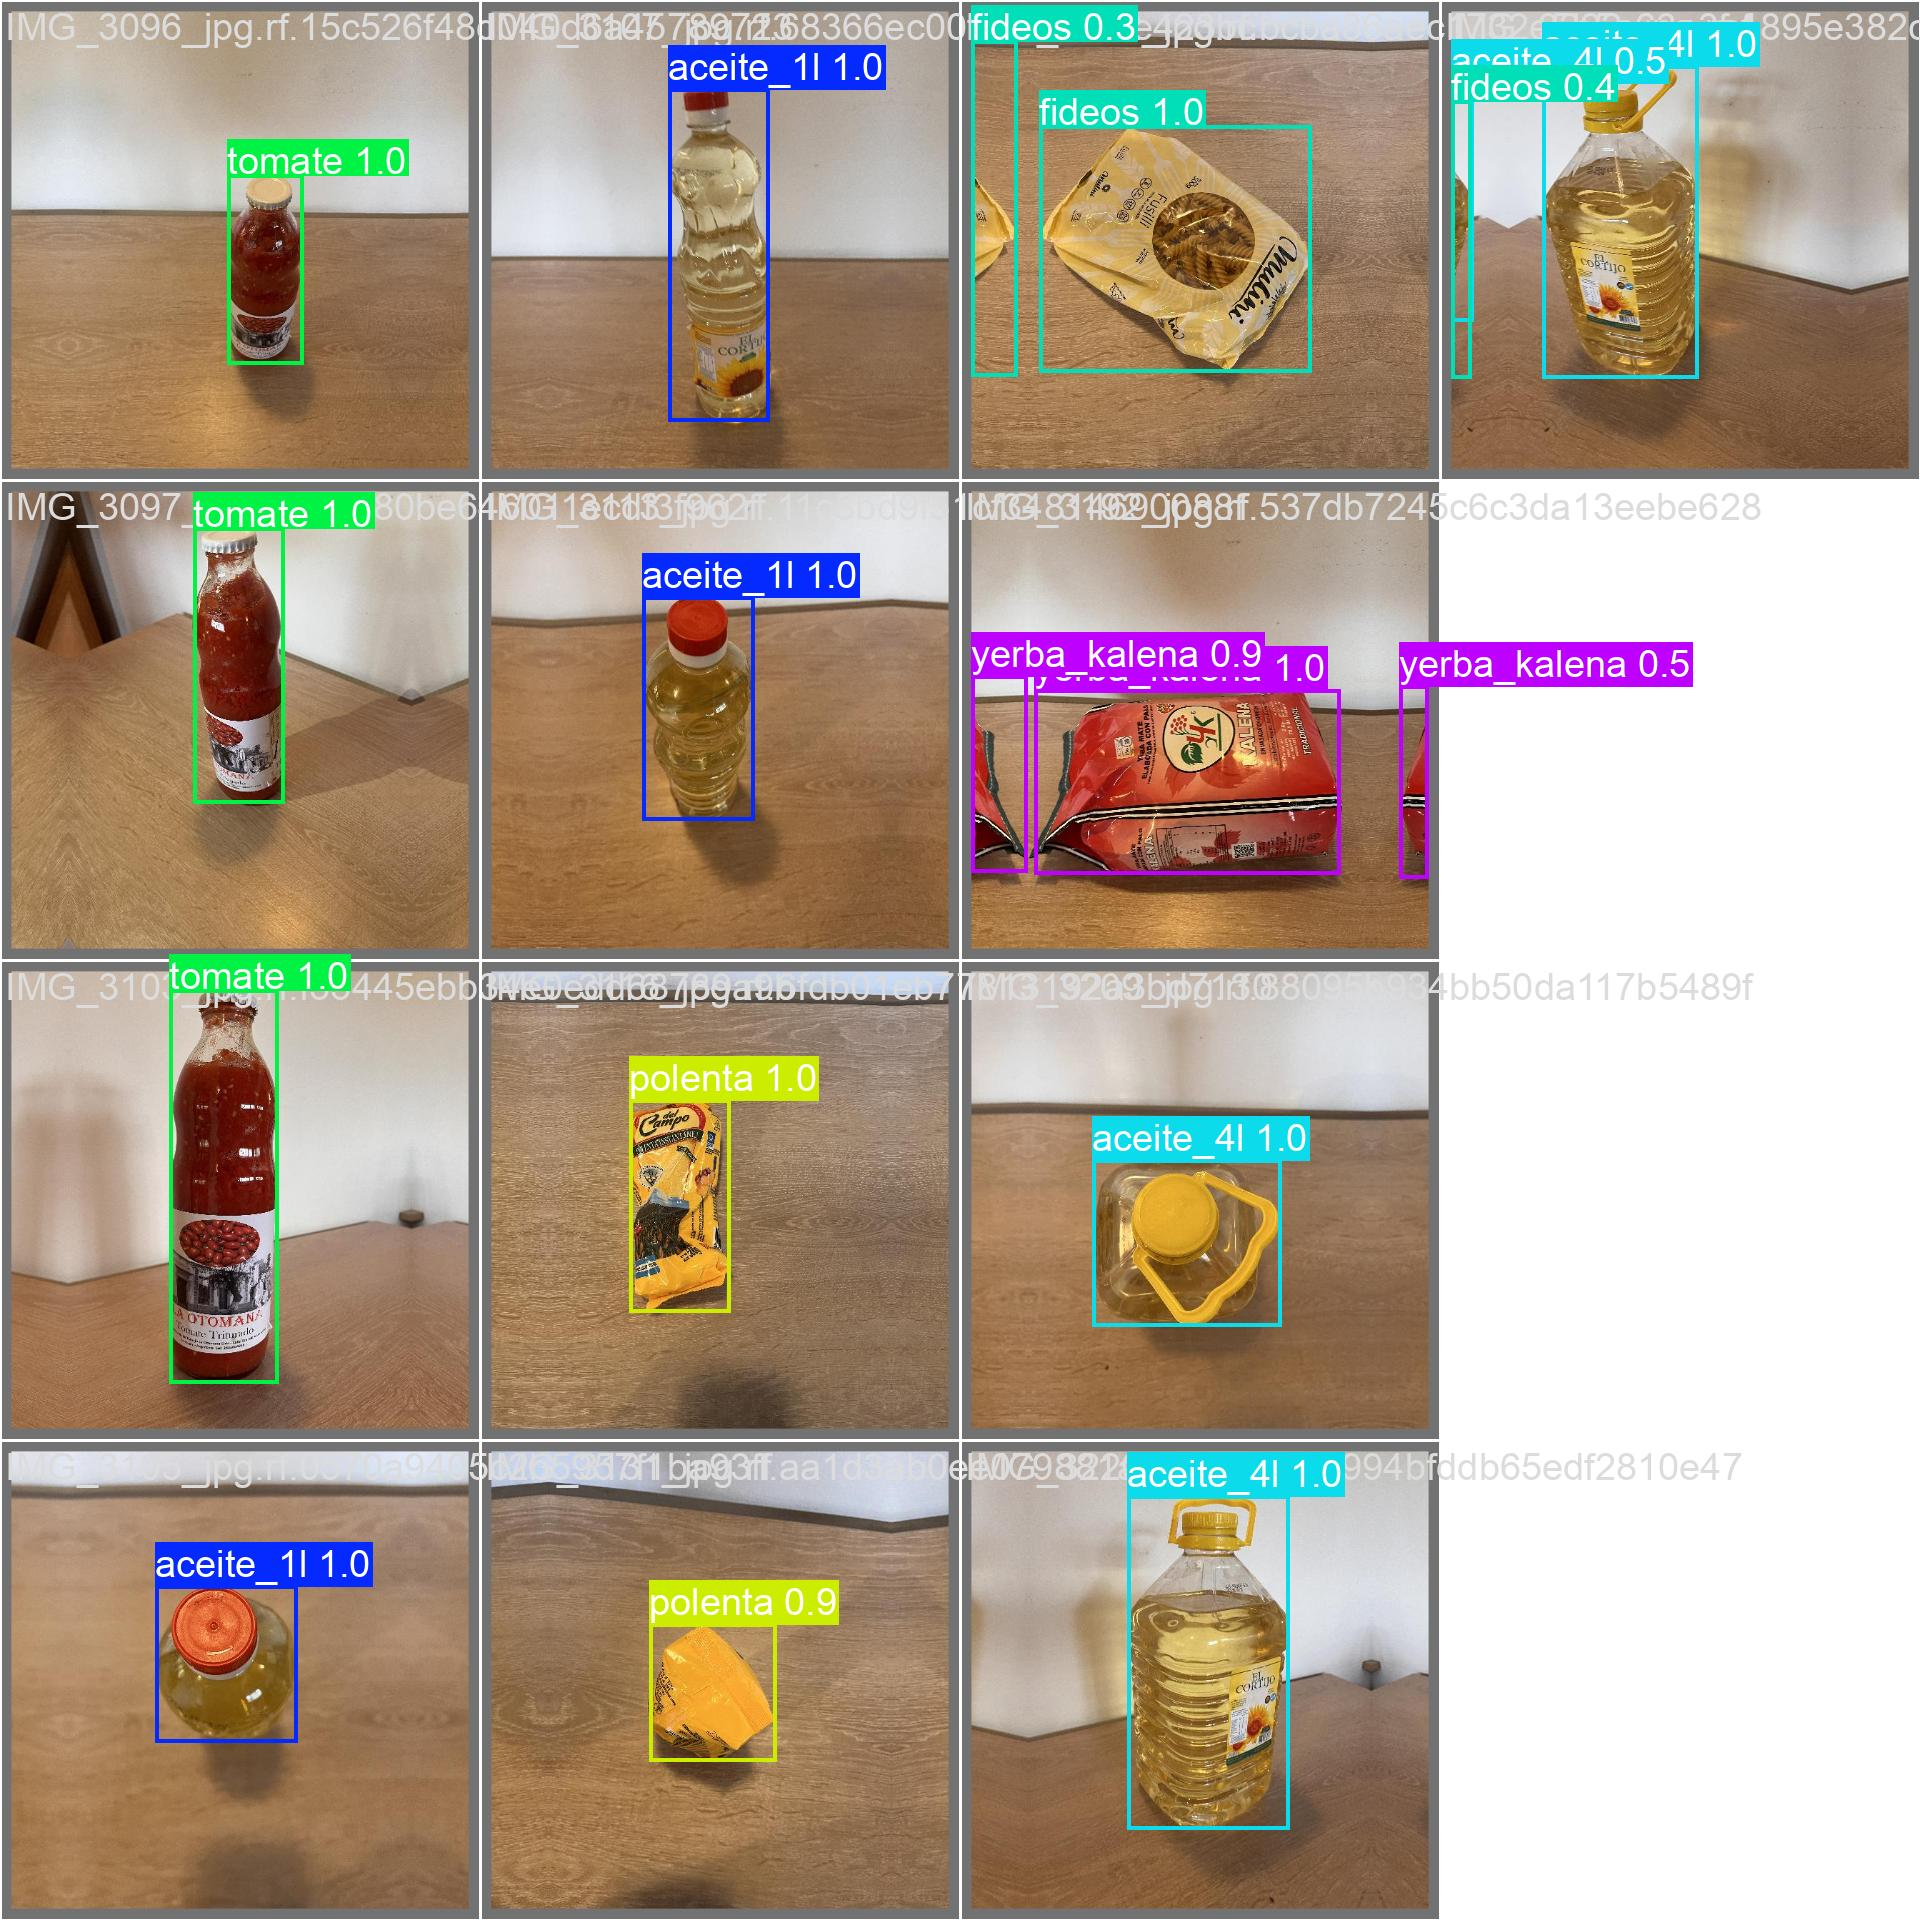
\includegraphics[width=\linewidth]{figures/val_batch0_pred.jpg}
  \caption{Ejemplos de predicciones (bounding boxes y nivel de confianza) generadas por YOLO11n.}
  \label{fig:val-pred}
\end{figure}


\subsection{Evaluación Final sobre Test Split (YOLO11n)}

Para validar la capacidad de generalización del modelo ganador (YOLO11n), se lo evaluó sobre un conjunto de test completamente independiente compuesto por 12 imágenes (20 instancias). Los resultados globales alcanzaron un mAP@0.5 de 0.833 y un mAP@0.5:0.95 de 0.755. La \cref{tab:resultados-test} presenta las métricas globales de esta evaluación.

\begin{table}[htbp]
\centering
\caption{Resultados de evaluación sobre Test Split --- YOLO11n.}
\label{tab:resultados-test}
\begin{tabular}{lc}
\hline
\textbf{Métrica} & \textbf{Valor} \\
\hline
mAP@0.5          & 0.833 \\
mAP@0.5:0.95     & 0.755 \\
Precision        & 0.620 \\
Recall           & 0.688 \\
\hline
\end{tabular}
\end{table}

El análisis de rendimiento por clases revela la alta sensibilidad de las métricas frente a datasets reducidos. Clases como \textit{aceite\_4l}, \textit{fideos}, \textit{miel} y \textit{tomate} lograron detecciones perfectas con un mAP@0.5 de 0.995. Destaca la inclusión de \textit{leche\_descremada} y \textit{miel}, las cuales no poseían representación en el split de validación, demostrando una sólida extracción de características por parte de la arquitectura.

\begin{figure}[htbp]
  \centering
  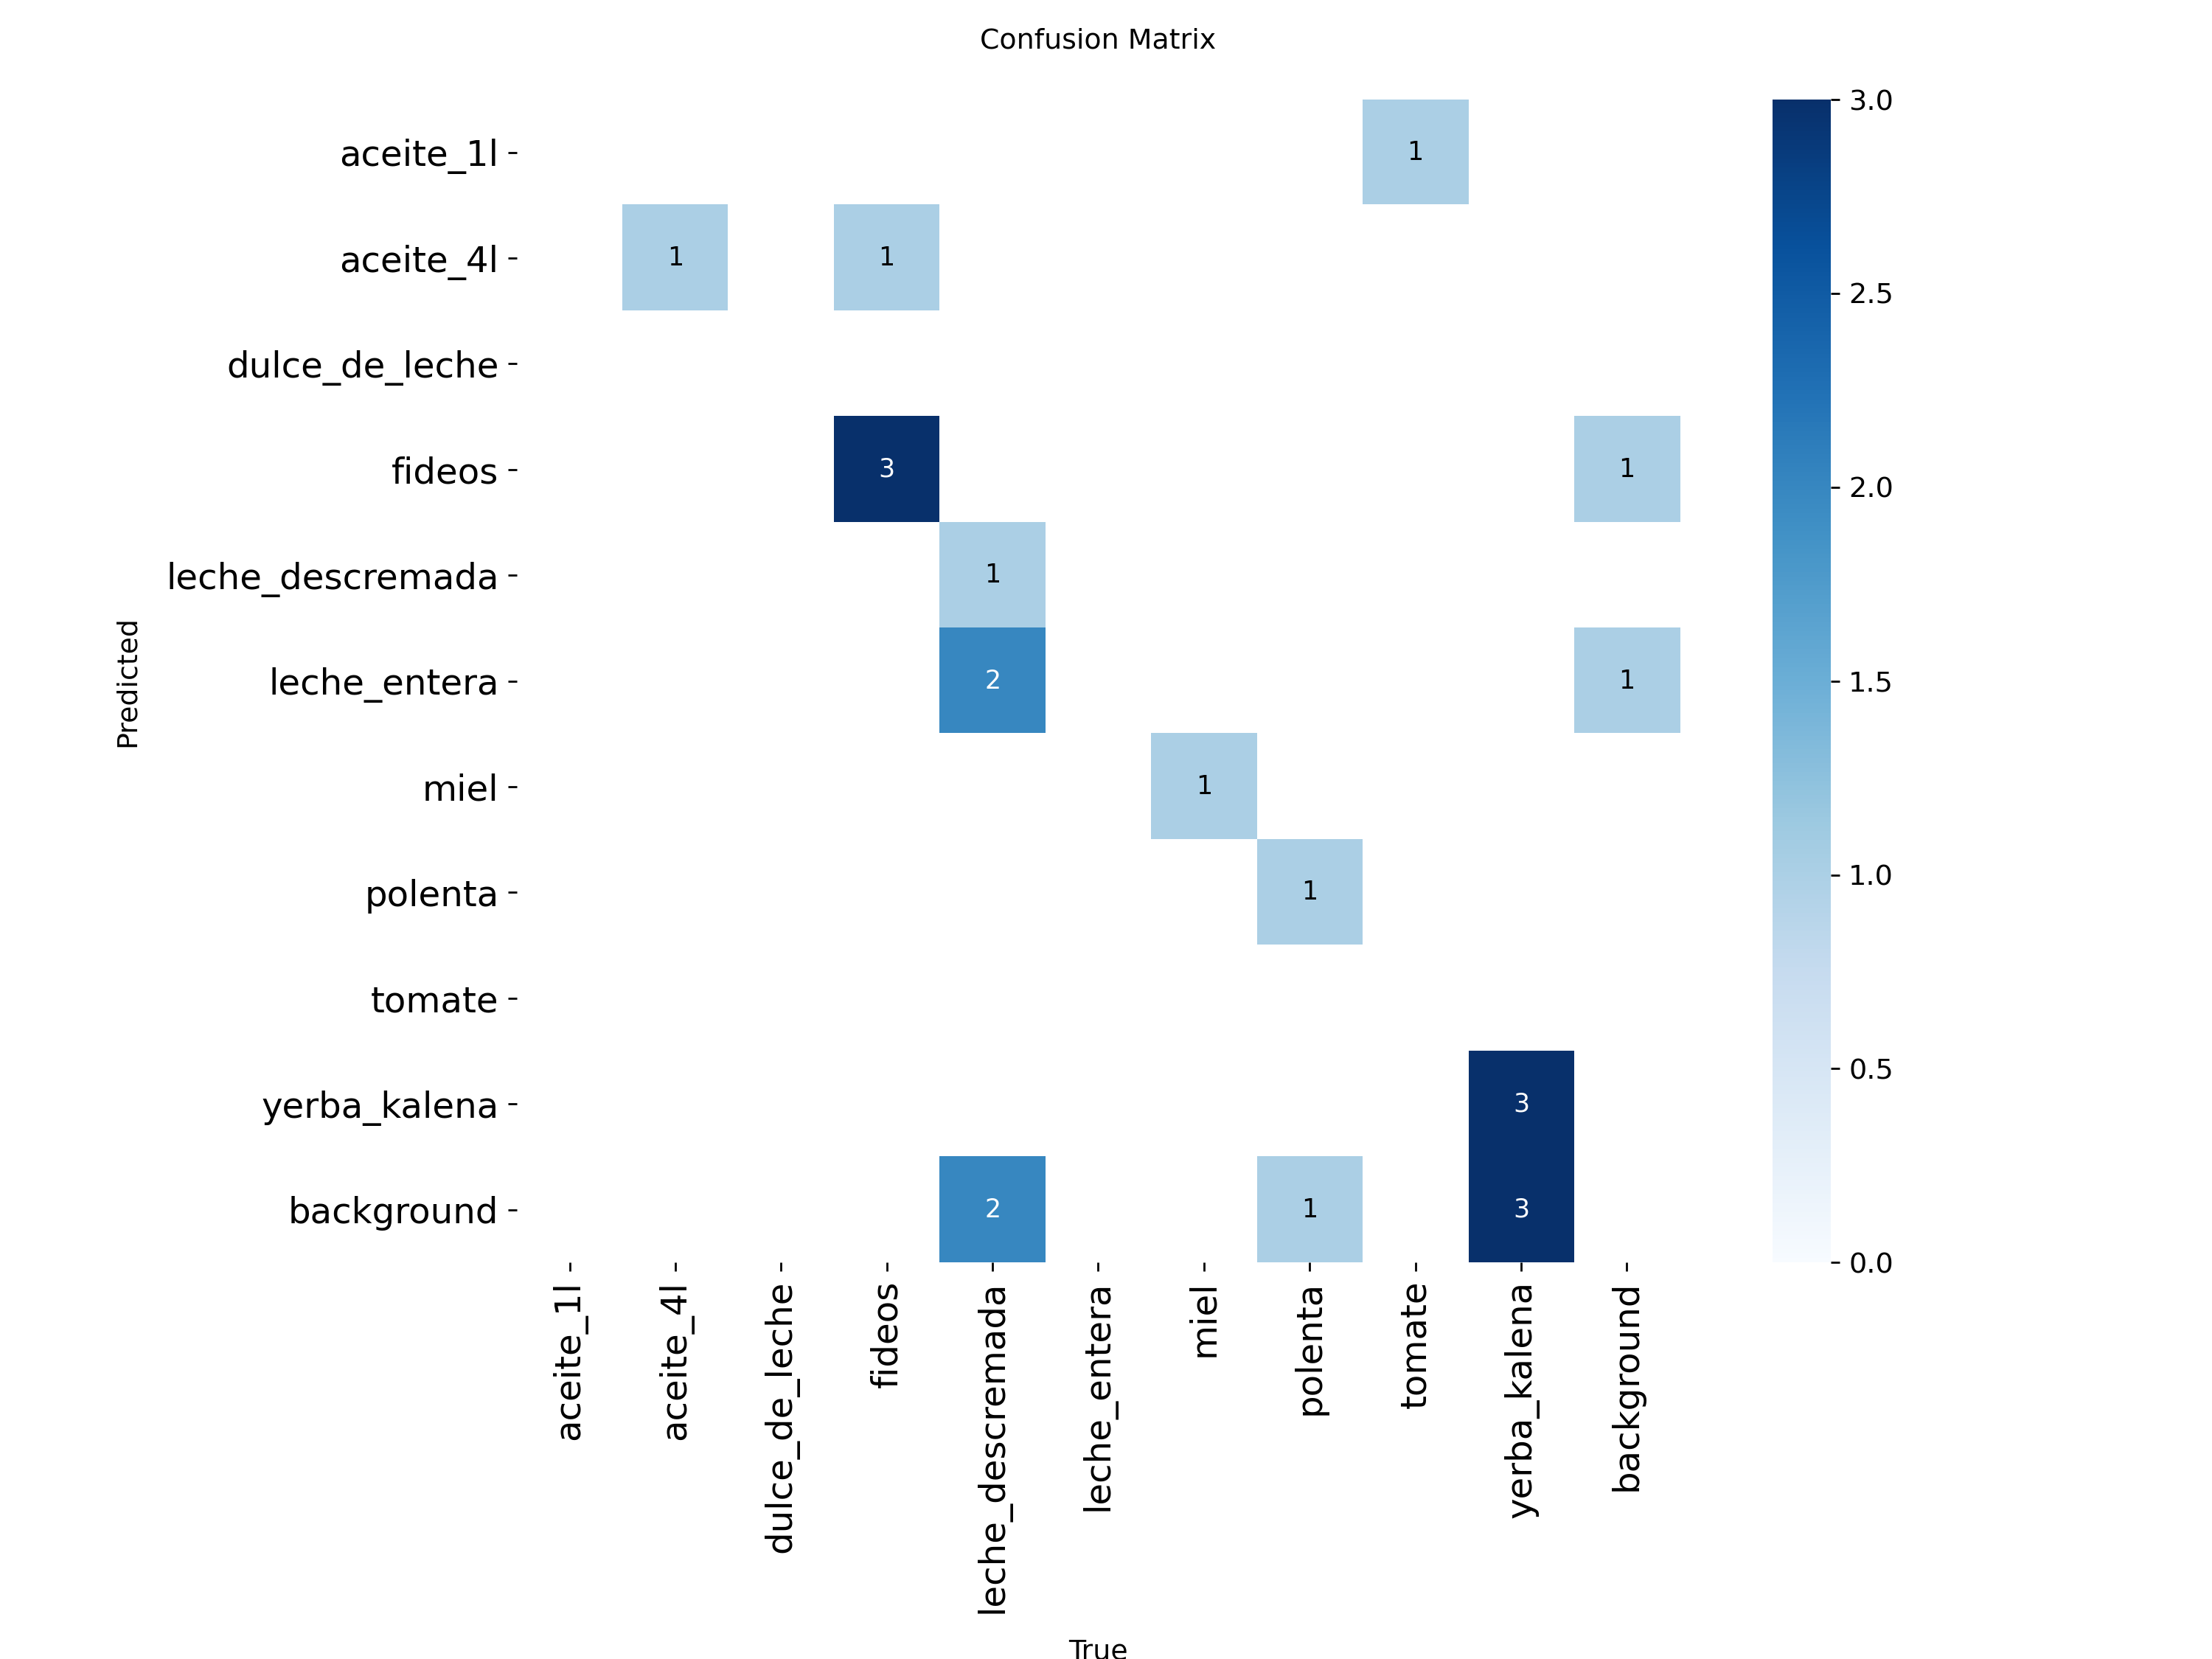
\includegraphics[width=\linewidth]{figures/test_confusion_matrix.png}
  \caption{Matriz de confusión para el modelo YOLO11n sobre el Test Split.}
  \label{fig:test-confusion-matrix}
\end{figure}

Por el contrario, como se observa en la matriz de confusión (\cref{fig:test-confusion-matrix}), \textit{polenta} y \textit{yerba\_kalena} registraron falsos negativos frente al fondo (background), bajando su rendimiento (mAP@0.5 de 0.495). Al contar con muy pocas instancias de estas clases en el conjunto de prueba, cualquier variación visual del envase impacta desproporcionadamente. 

\begin{figure}[htbp]
  \centering
  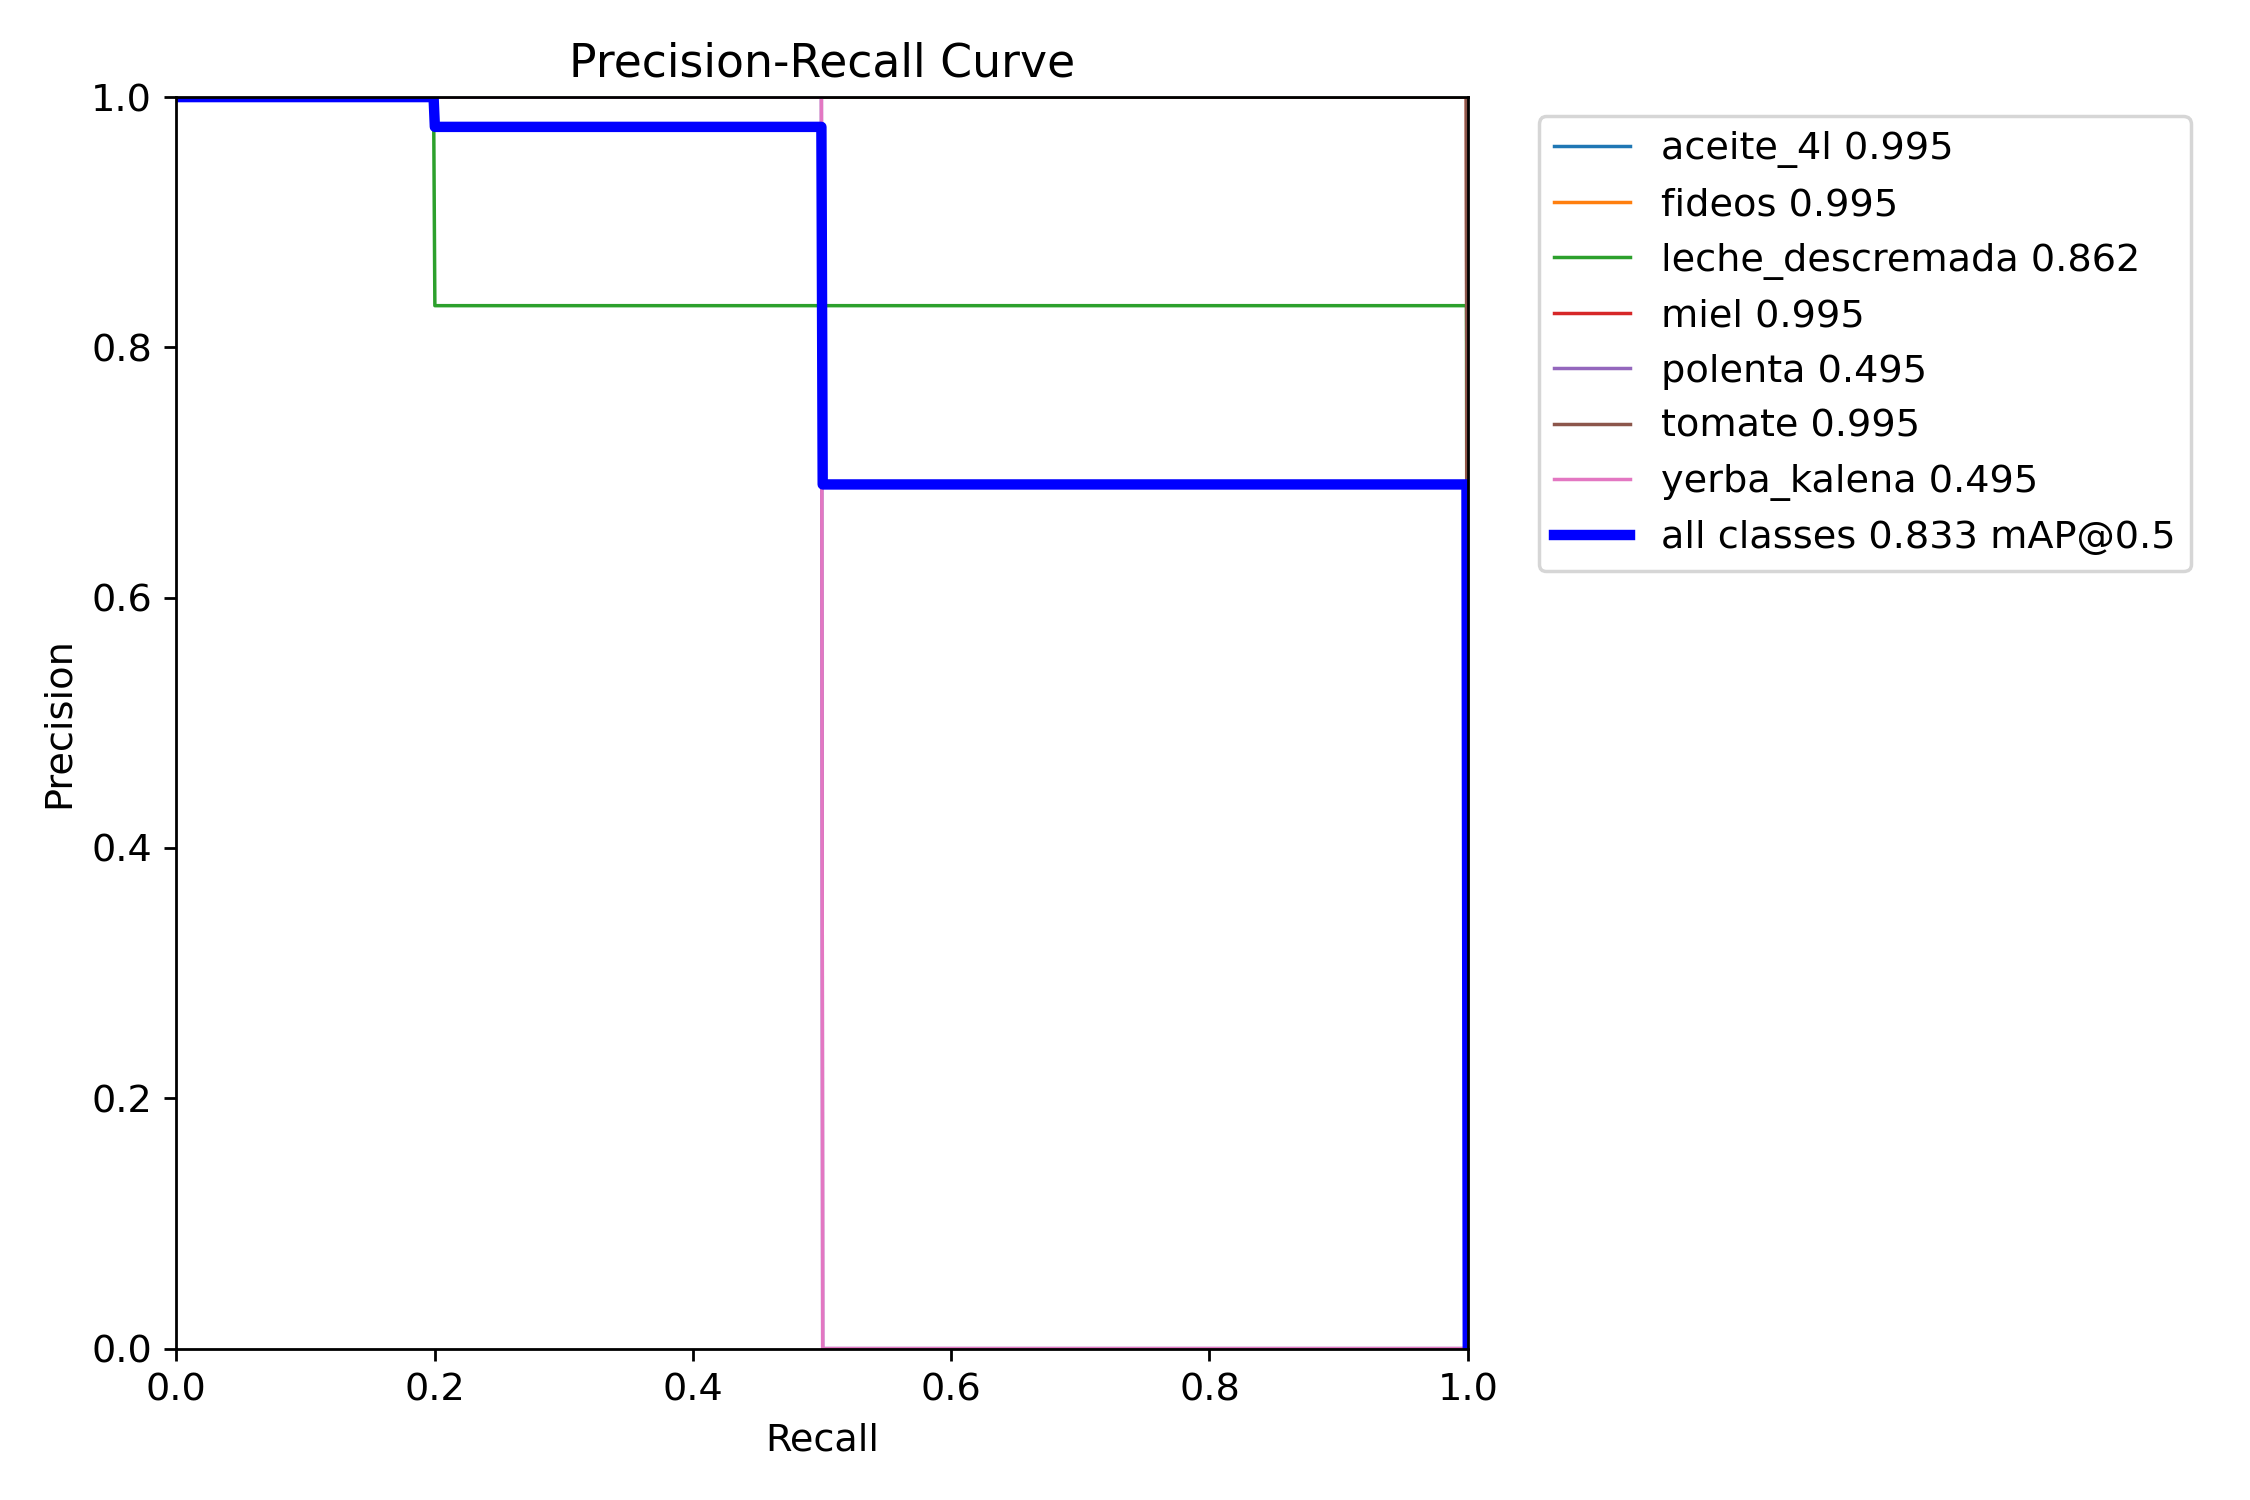
\includegraphics[width=\linewidth]{figures/test_PR_curve.png}
  \caption{Curvas Precision-Recall por clase sobre el Test Split. mAP@0.5 global = 0.833.}
  \label{fig:test-pr-curve}
\end{figure}

La \cref{fig:test-pr-curve} ilustra las curvas Precision-Recall de este examen final, consolidando a YOLO11n como un modelo robusto y preparado para escalar a un dataset de mayor volumen en la siguiente fase del proyecto.


\subsection{Rendimiento en Tiempo Real}

El sistema completo (captura de video + inferencia + tracking + visualización) opera a más de 15~FPS en la laptop de desarrollo. YOLO11n registró un tiempo de inferencia de 205.7~ms por imagen en el hardware de evaluación (Intel Core i5-6200U, CPU), siendo la arquitectura más rápida del benchmark. Para el hardware objetivo (Raspberry Pi~5, 8~GB), se estima un rendimiento de $\sim$10~FPS según los benchmarks del fabricante, valor operacionalmente viable dado que la velocidad de colocación de productos sobre la mesa por parte del usuario es significativamente menor.

\subsection{Demo End-to-End}

Se validó el sistema completo con un escenario simulado de checkout: partiendo de una mesa vacía, se agregaron productos de a uno, verificando la correcta confirmación multi-frame, la acumulación en el panel lateral y la generación del archivo JSON de salida. El sistema registró correctamente todos los productos colocados, sin duplicaciones y sin falsos positivos persistentes.

\subsection{Impacto del Data Augmentation}

Para cuantificar el impacto del data augmentation en la generalización del modelo, se compararon tres estrategias de augmentation entrenando YOLO11n sobre el dataset multi-producto con idéntica configuración (100 épocas, seed fija para reproducibilidad). Los resultados se presentan en la \cref{tab:augmentation}.

\begin{table}[htbp]
\centering
\caption{Comparación de estrategias de data augmentation --- YOLO11n sobre dataset multi-producto.}
\label{tab:augmentation}
\begin{tabular}{lcccc}
\hline
\textbf{Configuración} & \textbf{Val mAP@0.5} & \textbf{Test mAP@0.5} & \textbf{Test P} & \textbf{Test R} \\
\hline
Sin augmentation       & 0.851 & 0.693 & 0.878 & 0.481 \\
Default Ultralytics    & \textbf{0.946} & \textbf{0.820} & \textbf{0.874} & \textbf{0.671} \\
Augmentation agresivo  & 0.606 & 0.641 & 0.628 & 0.619 \\
\hline
\end{tabular}
\end{table}

Los resultados confirman que el data augmentation es crítico para la generalización: sin augmentation, el rendimiento en test cae significativamente. La configuración por defecto de Ultralytics (mosaic, flip horizontal, jitter HSV) ofrece el mejor balance entre precision y recall, superando tanto a la ausencia de augmentation como a la configuración agresiva (que incorpora mixup, rotación de 15 grados y jitter HSV más intenso).

%% ===========================================================================
\section{Discusión}
\label{sec:discusion}

\subsection{Interpretación de Resultados}

YOLO11n alcanzó un mAP@0.5 de 0.967 en validación sobre el dataset de producto individual (10 clases), superando ampliamente el umbral mínimo de 0.70 definido en la planificación. En el test split independiente, el modelo obtuvo un mAP@0.5 de 0.833, confirmando la capacidad de generalización. La diferencia entre validación y test (13.4 puntos) sugiere cierto overfitting atribuible al tamaño reducido del dataset. Si bien la comparación directa con el dataset RPC~\cite{wei2019rpc} (que reporta mAP entre 0.50 y 0.80 sobre 200 categorías) no es directa por la diferencia de escala, los resultados confirman la viabilidad del enfoque para un catálogo acotado.

\subsection{Limitaciones}

El presente trabajo tiene las siguientes limitaciones:
\begin{itemize}
  \item \textbf{Escala del dataset:} Solo se evaluaron 10 de las $\sim$60 clases del catálogo completo de la despensa, con un total de 296 imágenes anotadas.
  \item \textbf{Condiciones controladas:} Las imágenes se capturaron bajo iluminación y fondo uniformes. No se evaluó el rendimiento bajo condiciones de iluminación variable.
  \item \textbf{Diferencia validación-test:} El gap de 13.4 puntos de mAP@0.5 entre validación (0.967) y test (0.833) sobre el dataset individual sugiere overfitting por el tamaño reducido del dataset, mitigable con mayor cantidad de imágenes.
  \item \textbf{Métricas de sistema pendientes:} No se midieron métricas end-to-end (order-level accuracy, duplicate rate, miss rate) sobre un benchmark estandarizado.
\end{itemize}

\subsection{Trabajo Futuro}

Las líneas de trabajo futuro incluyen: (1)~escalar el dataset a las $\sim$60 clases del catálogo completo, manteniendo el mismo protocolo de captura y augmentation; (2)~definir métricas de sistema end-to-end (order-level accuracy, duplicate rate, miss rate) sobre un benchmark estandarizado; (3)~evaluar el rendimiento bajo condiciones de iluminación variable y fondos no controlados; (4)~desplegar el sistema en Raspberry Pi~5 para validación en condiciones reales de operación; y (5)~integrar el módulo de detección con el sistema de gestión de la mutual para automatizar el cobro.

%% ===========================================================================
\section{Conclusiones}
\label{sec:conclusiones}

A partir del diseño, implementación y evaluación del sistema de autocobro propuesto, se derivan las siguientes conclusiones:

\begin{enumerate}
  \item El benchmark comparativo entre YOLOv8n, YOLOv10n y YOLO11n determinó que YOLO11n ofrece el mejor balance precisión-velocidad, alcanzando un mAP@0.5 de 0.967 en validación y 0.833 en test sobre el dataset individual (10 clases), superando el umbral mínimo de 0.70 y confirmando la viabilidad del enfoque single-stage para este dominio.

  \item La arquitectura single-stage con YOLO11n (2.5M parámetros) permite inferencia en tiempo real superior a 15~FPS en laptop y $\sim$10~FPS en Raspberry Pi~5, cumpliendo los requisitos de latencia para una experiencia de usuario fluida sin requerir hardware especializado.

  \item La lógica de registro multi-frame basada en IoU, con confirmación a 5 frames y tolerancia de desaparición de 10 frames, demostró ser efectiva para suprimir falsos positivos sin introducir latencia perceptible, ofreciendo una alternativa simple y robusta frente a trackers más complejos como ByteTrack para el caso de uso de productos estacionarios.

  \item El data augmentation resultó crítico para la generalización del modelo: sin augmentation, el rendimiento en test cae significativamente (ver \cref{tab:augmentation}). Las técnicas por defecto de Ultralytics (mosaic, flip horizontal, jitter HSV) ofrecen el mejor balance, superando tanto la ausencia de augmentation como configuraciones más agresivas.

  \item La diferencia de 13.4 puntos entre validación y test (0.967 vs. 0.833) sobre el dataset individual evidencia overfitting atribuible al tamaño reducido del dataset (296 imágenes). Escalar a las $\sim$60 clases del catálogo completo con mayor cantidad de imágenes por clase es la principal línea de trabajo futuro para mejorar la capacidad de generalización.

  \item La metodología propuesta es reproducible y extensible: el mismo protocolo de captura, pipeline de augmentation y arquitectura de modelo pueden aplicarse para escalar el catálogo sin cambios en la arquitectura del sistema. El código fuente y los datasets se encuentran disponibles públicamente.

  \item Los resultados validan la viabilidad de un sistema de autocobro basado exclusivamente en visión por computadora como alternativa de bajo costo para organizaciones comunitarias, sin requerir sensores adicionales, infraestructura de nube ni soluciones comerciales costosas.
\end{enumerate}

\section*{Agradecimientos}

Los autores agradecen a los profesores de la materia Visión por Computadora~II de la Carrera de Especialización en Inteligencia Artificial (CEIA), Facultad de Ingeniería, Universidad de Buenos Aires, por la orientación y los recursos proporcionados durante el desarrollo de este trabajo.

% Bibliography
\bibliographystyle{IEEEtranN}
\bibliography{paper}

\end{document}
